% !TEX program = xelatex
\documentclass[a4paper,11.5pt,UTF8]{ctexart}
\usepackage{a4}
\usepackage{amsmath, amssymb, amsthm, graphicx, xspace,array,url}
\usepackage{setspace}
\usepackage{float}
\usepackage{listings,color,xcolor,fontspec}

\CTEXsetup[format={\Large\bfseries}]{section}

\title{Project 2}
\author{张卓涵 3190101161}
\usepackage[a4paper,left=20mm,right=20mm,top=30mm,bottom=20mm]{geometry}

\newtheorem{example}{\hspace{2em}例}{}
\newtheorem{remark}{\hspace{2em}注}{}
\newtheorem{thm}{\hspace{2em}定理}{}
\newtheorem{lemma}{\hspace{2em}引理}{}

\begin{document}
\begin{figure}[t]
\begin{minipage}[h]{0.25\linewidth}
	
\includegraphics[width=4.0cm]{./figure/ZJU2.jpeg}
\end{minipage}
\hfill
\begin{minipage}[h]{.7\linewidth}
	\begin{flushright}
			\Large{微分方程数值解
				\vspace{3mm}	\\
				   2022 夏
				\vspace{3mm}	\\
				   张卓涵 \hspace{3mm}3190101161}
	\end{flushright}
\end{minipage}
\rule{\linewidth}{0.1em}
\end{figure}
\begin{center}
	\huge{\textbf{Project 2}}
\end{center}
\begin{large}
	
\section{Declaration}
\par 本次作业选择的边值类型是Dirichlet与Neumann混合,V-cycle会执行二三十次才能达到预计的精度,如果是纯Dirichlet条件一般只需执行6、7次即可。考虑到为了不使作业文件显得过于冗杂,这里不再针对纯Dirichlet条件进行一套相似的实验和分析。
	
\section{Assignment.A}
\par 笔者选择了三个不同的一元函数,分别对三个函数的(b,c,d)的所有不同组合做了测试。考虑篇幅限制,报告文档里只展示restriction算子为full weighting,prolongation算子为linear时的部分数值结果,完整数值结果见于output目录下的OneDimGrid.txt文件.
\par 选取的边值条件为半Neumann半Dirichlet.
\subsection{1st function}
\par 第一个函数是$$f(x)=\exp\{\sin(\pi x)\}$$
当$n=32$时,
\begin{center}
	\begin{tabular}{|c|c|c|c|}
		\hline
		 & 残差 & 与解析解误差 & 与离散解误差 \\
		\hline
		FMG & 0.68723 & 0.167923 & 0.165495 \\
		\hline
		22次V-cycle & 8.32581e-08 & ~ & ~ \\
		\hline
		23次V-cycle & 3.57647e-08 & ~ & ~ \\
		\hline
		24次V-cycle & 1.53634e-08 & ~ & ~ \\
		\hline
		25次V-cycle & 6.59929e-09 & 0.00423999 & 1.60286e-09 \\
		\hline
	\end{tabular}
\end{center}
当$n=64$时,
\begin{center}
	\begin{tabular}{|c|c|c|c|}
		\hline
		& 残差 & 与解析解误差 & 与离散解误差 \\
		\hline
		FMG & 0.325315 & 0.0699889 & 0.0696978 \\
		\hline
		23次V-cycle & 8.54498e-08 & ~ & ~ \\
		\hline
		24次V-cycle & 3.70082e-08 & ~ & ~ \\
		\hline
		25次V-cycle & 1.6028e-08 & ~ & ~ \\
		\hline
		26次V-cycle & 6.94126e-09 & 0.000894427 & 1.19759e-09 \\
		\hline
	\end{tabular}
\end{center}
当$n=128$时,
\begin{center}
	\begin{tabular}{|c|c|c|c|}
		\hline
		& 残差 & 与解析解误差 & 与离散解误差 \\
		\hline
		FMG & 0.173425 & 0.0278183 & 0.0277827 \\
		\hline
		24次V-cycle & 8.29168e-08 & ~ & ~ \\
		\hline
		25次V-cycle & 3.61615e-08 & ~ & ~ \\
		\hline
		26次V-cycle & 1.5767e-08 & ~ & ~ \\
		\hline
		27次V-cycle & 6.8685e-09 & 0.000204596 & 8.39315e-10 \\
		\hline
	\end{tabular}
\end{center}
当$n=256$时,
\begin{center}
	\begin{tabular}{|c|c|c|c|}
		\hline
		& 残差 & 与解析解误差 & 与离散解误差 \\
		\hline
		FMG & 0.0950385 & 0.010416 & 0.0104116 \\
		\hline
		25次V-cycle & 7.73434e-08 & ~ & ~ \\
		\hline
		26次V-cycle & 3.39351e-08 & ~ & ~ \\
		\hline
		27次V-cycle & 1.49012e-08 & ~ & ~ \\
		\hline
		28次V-cycle & 6.54836e-09 & 4.88739e-05 & 5.62325e-10 \\
		\hline
	\end{tabular}
\end{center}
可以看到,每进行一次V-cycle,残差约减小为原先的$\frac{1}{2}$.
\par 绘制在$n=256$时求解出的函数图像为:
\begin{figure}[H]
	\centering
	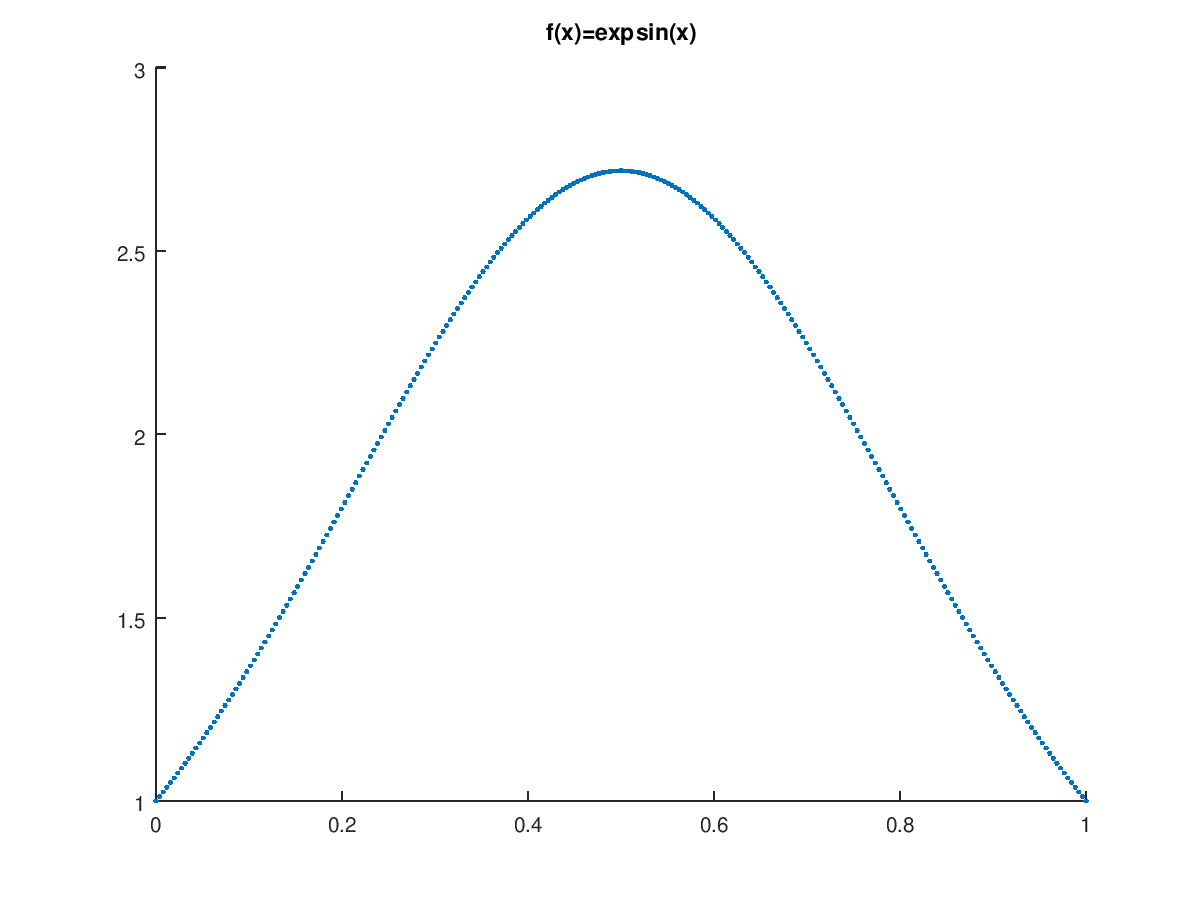
\includegraphics[width=0.8\textwidth,height=0.6\textwidth]{../output/figure/dim1_1.png}
\end{figure}

\subsection{2nd function}
\par 第二个函数是:$$f(x)=x^2-x$$
简便起见,仅展示$n=256$时的数值结果如下:
\begin{center}
	\begin{tabular}{|c|c|c|c|}
		\hline
		& 残差 & 与解析解误差 & 与离散解误差 \\
		\hline
		FMG & 0.0493678 & 0.0011591 & 0.0011591 \\
		\hline
		24次V-cycle & 5.60557e-08 & ~ & ~ \\
		\hline
		25次V-cycle & 2.45878e-08 & ~ & ~ \\
		\hline
		26次V-cycle & 1.0785e-08 & ~ & ~ \\
		\hline
		27次V-cycle & 4.73068e-09 & 4.07266e-10 & 4.07266e-10 \\
		\hline
	\end{tabular}
\end{center}
可以看到,每进行一次V-cycle,残差约减小为原先的$\frac{1}{2}$.
\par 绘制在$n=256$时求解出的函数图像为:
\begin{figure}[H]
	\centering
	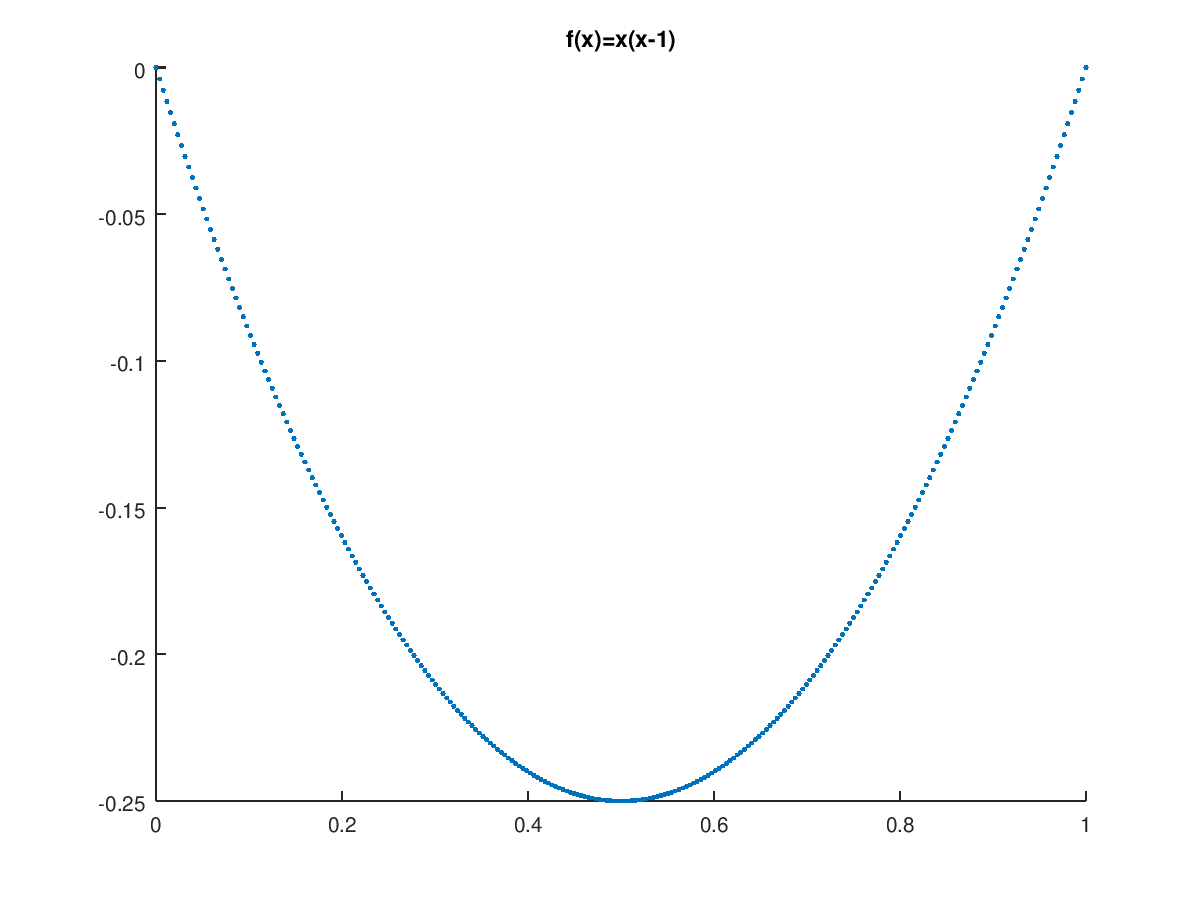
\includegraphics[width=0.8\textwidth,height=0.6\textwidth]{../output/figure/dim1_2.png}
\end{figure}

\subsection{3rd function}
\par 第三个函数是:$$f(x)=\frac{1}{x+1}$$
简便起见,仅展示$n=256$时的数值结果如下:
\begin{center}
	\begin{tabular}{|c|c|c|c|}
		\hline
		& 残差 & 与解析解误差 & 与离散解误差 \\
		\hline
		FMG & 0.0439872 & 0.00116783 & 0.0012034 \\
		\hline
		24次V-cycle & 7.62302e-08 & ~ & ~ \\
		\hline
		25次V-cycle & 3.3433e-08 & ~ & ~ \\
		\hline
		26次V-cycle & 1.46611e-08 & ~ & ~ \\
		\hline
		27次V-cycle & 6.43922e-09 & 3.55659e-05 & 5.53656e-10 \\
		\hline
	\end{tabular}
\end{center}
可以看到,每进行一次V-cycle,残差约减小为原先的$\frac{1}{2}$.
\par 绘制在$n=256$时求解出的函数图像为:
\begin{figure}[H]
	\centering
	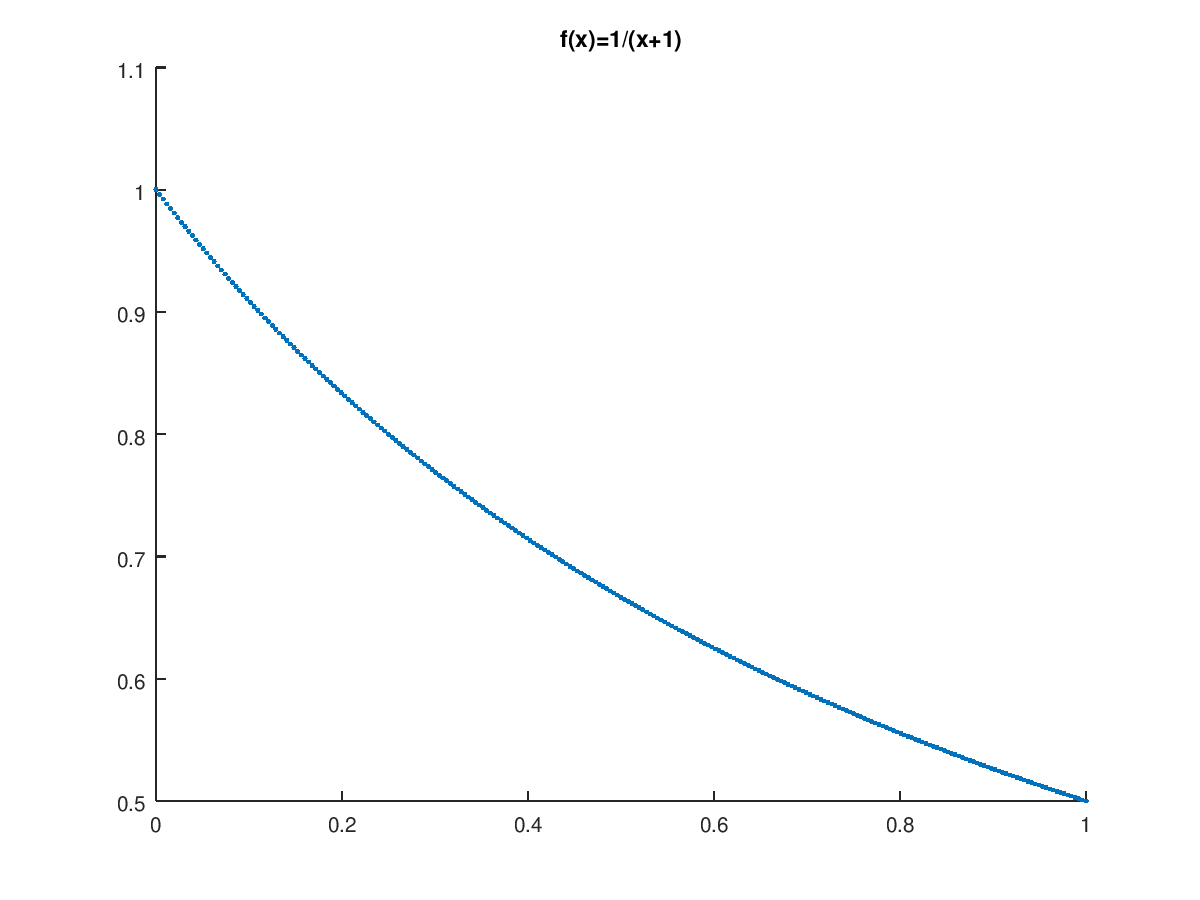
\includegraphics[width=0.8\textwidth,height=0.6\textwidth]{../output/figure/dim1_3.png}
\end{figure}

\subsection{convergence rate of error vector}
通过./output/OneDimGrid.txt中的函数error\_convergence()的输出结果看到误差向量的收敛率与残差相近,即每进行一次V-cycle,约减小一半.

\subsection{Section 9.5.1 \uppercase\expandafter{\romannumeral3}}
\begin{center}
	\begin{tabular}{|c|c|c|c|c|c|c|}
		\hline
		 & $\epsilon=10^{-8}$ & $\epsilon=10^{-9}$ & $\epsilon=10^{-10}$ & $\epsilon=10^{-11}$ & $\epsilon=10^{-12}$ & $\epsilon=10^{-13}$ \\
		 \hline
		 V-cycle次数 & 26 & 29 & 32 & 35 & $\infty$ & $\infty$ \\
		 \hline
	\end{tabular}
\end{center}
当$\epsilon$下降至$10^{-12}$量级时,程序不再能达到预设的精度,这可能的原因是机器误差导致的.

\section{Assignment.B}
\par 笔者选择了三个不同的二元函数,分别对三个函数的(b,c,d)的所有不同组合做了测试。考虑篇幅限制,报告文档里只展示restriction算子为full weighting,prolongation算子为linear时的部分数值结果,完整数值结果见于output目录下的TwoDimGrid.txt文件.
\par 选取的边值条件为左边界是Neumann半,其他三个边界是Dirichlet.
\par 考虑到对二维网格计算离散准确解误差从时间和空间上来说都极其耗费资源,于是实验中只对第一个函数计算了算子为full weighting和linear时,$n=32,64,128$时的离散误差.

\subsection{1st function}
\par 第一个函数是:$$f(x,y)=e^{y+\sin(x)}$$
当$n=32$时,
\begin{center}
	\begin{tabular}{|c|c|c|c|}
		\hline
		& 残差 & 与解析解误差 & 与离散解误差 \\
		\hline
		FMG & 0.5156 & 0.00432243 & 0.00435407 \\
		\hline
		22次V-cycle & 1.11125e-07 & ~ & ~ \\
		\hline
		23次V-cycle & 4.52073e-08 & ~ & ~ \\
		\hline
		24次V-cycle & 1.83927e-08 & ~ & ~ \\
		\hline
		25次V-cycle & 7.4815e-09 & 4.36528e-05 & 2.08002e-10 \\
		\hline
	\end{tabular}
\end{center}
当$n=64$时,
\begin{center}
	\begin{tabular}{|c|c|c|c|}
		\hline
		& 残差 & 与解析解误差 & 与离散解误差 \\
		\hline
		FMG & 0.521522 & 0.00263346 & 0.00264354 \\
		\hline
		26次V-cycle & 8.80354e-08 & ~ & ~ \\
		\hline
		27次V-cycle & 3.98431e-08 & ~ & ~ \\
		\hline
		28次V-cycle & 1.80335e-08 & ~ & ~ \\
		\hline
		29次V-cycle & 8.15999e-09 & 1.16245e-05 & 1.60224e-10 \\
		\hline
	\end{tabular}
\end{center}
当$n=128$时,
\begin{center}
	\begin{tabular}{|c|c|c|c|}
		\hline
		& 残差 & 与解析解误差 & 与离散解误差 \\
		\hline
		FMG & 0.523524 & 0.00163054 & 0.00163332 \\
		\hline
		30次V-cycle & 6.17438e-08 & ~ & ~ \\
		\hline
		31次V-cycle & 3.00788e-08 & ~ & ~ \\
		\hline
		32次V-cycle & 1.46829e-08 & ~ & ~ \\
		\hline
		33次V-cycle & 7.15954e-09 & 3.00383e-06 & 1.19028e-09 \\
		\hline
	\end{tabular}
\end{center}
当$n=256$时,
\begin{center}
	\begin{tabular}{|c|c|c|}
		\hline
		& 残差 & 与解析解误差  \\
		\hline
		FMG & 0.524378 & 0.00102629  \\
		\hline
		34次V-cycle & 3.9814e-08 & ~  \\
		\hline
		35次V-cycle & 2.05473e-08 & ~  \\
		\hline
		36次V-cycle & 1.05356e-08 & ~  \\
		\hline
		37次V-cycle & 5.47152e-09 & 7.63851e-07  \\
		\hline
	\end{tabular}
\end{center}
可以看到,每进行一次V-cycle,残差减小到原先的$\frac{1}{2}$.
\par 绘制出在$n=64$时求解的函数图像为:
\begin{figure}[H]
	\centering
	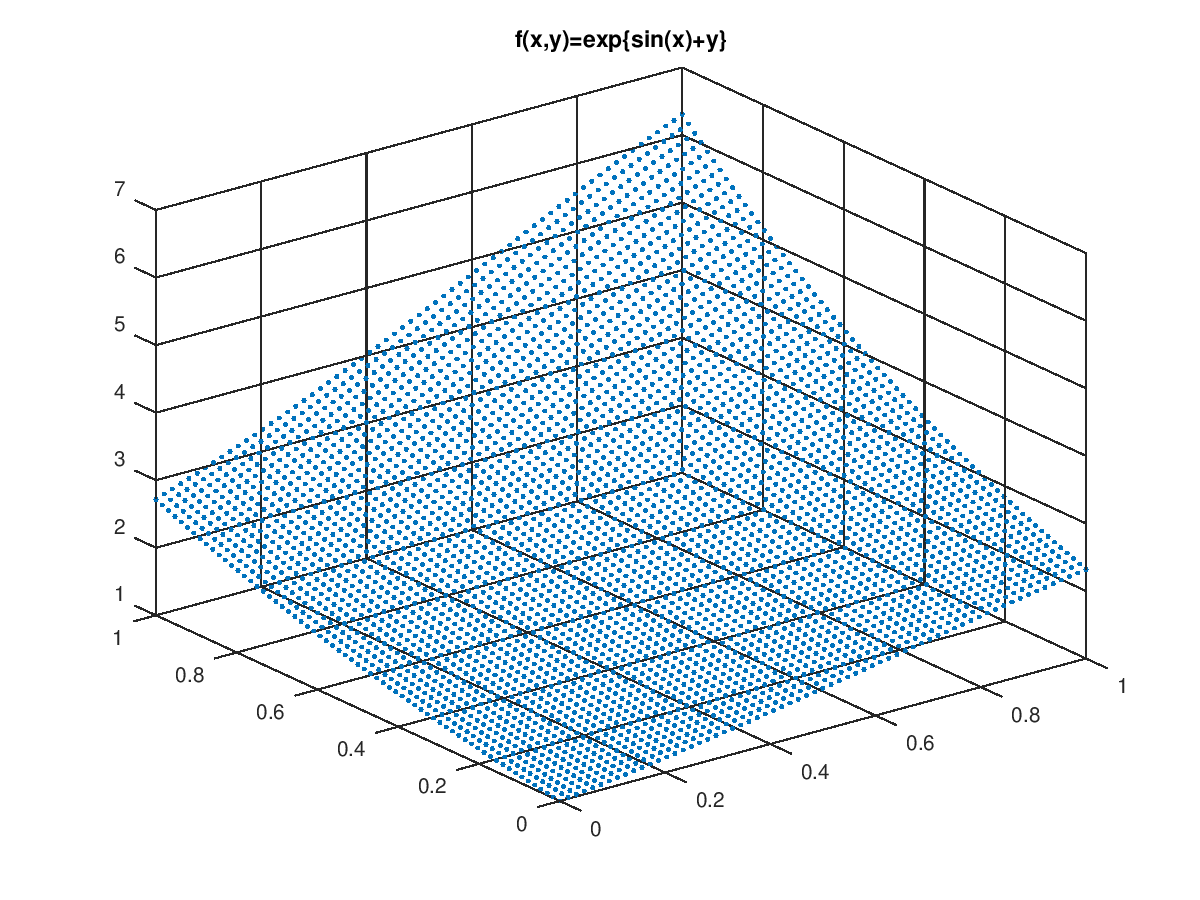
\includegraphics[width=0.8\textwidth,height=0.6\textwidth]{../output/figure/dim2_1.png}
\end{figure}

\subsection{2nd function}
\par 第二个函数是:$$f(x,y)=x^2+y^2$$
简便起见,仅展示$n=256$时的数值结果:
\begin{center}
	\begin{tabular}{|c|c|c|}
		\hline
		& 残差 & 与解析解误差  \\
		\hline
		FMG & 0.38627 & 0.0011954  \\
		\hline
		26次V-cycle & 6.07797e-08 & ~  \\
		\hline
		27次V-cycle & 3.06209e-08 & ~  \\
		\hline
		28次V-cycle & 1.54287e-08 & ~  \\
		\hline
		29次V-cycle & 7.778e-09 & 3.80175e-11  \\
		\hline
	\end{tabular}
\end{center}
可以看到,每进行一次V-cycle,残差减小到原先的$\frac{1}{2}$.
\par 绘制出在$n=64$时求解的函数图像为:
\begin{figure}[H]
	\centering
	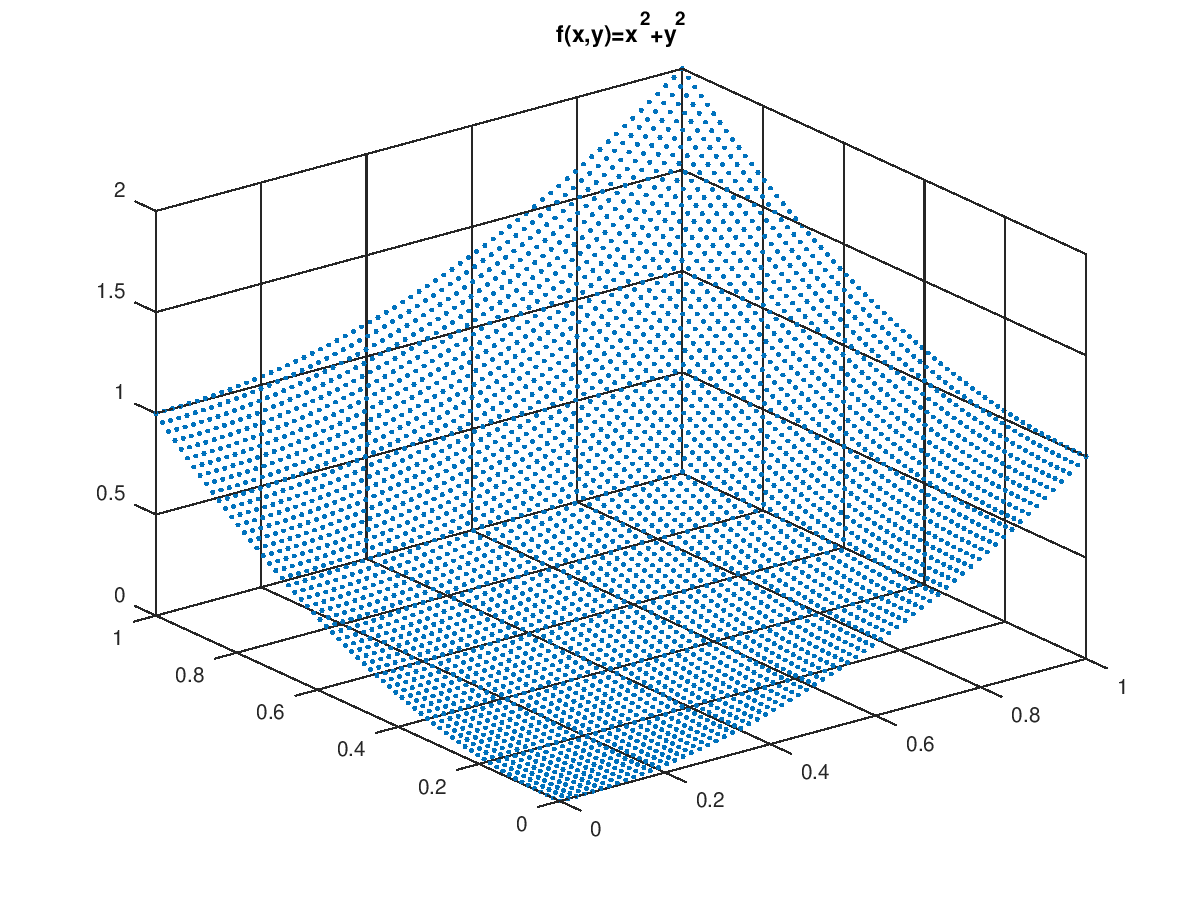
\includegraphics[width=0.8\textwidth,height=0.6\textwidth]{../output/figure/dim2_2.png}
\end{figure}

\subsection{3rd function}
\par 第三个函数是:$$f(x,y)=sin(x+y)$$
简便起见,仅展示$n=256$时的数值结果:
\begin{center}
	\begin{tabular}{|c|c|c|}
		\hline
		& 残差 & 与解析解误差  \\
		\hline
		FMG & 0.162152 & 0.000228387  \\
		\hline
		33次V-cycle & 3.881e-08 & ~  \\
		\hline
		34次V-cycle & 1.99943e-08 & ~  \\
		\hline
		35次V-cycle & 1.03028e-08 & ~  \\
		\hline
		36次V-cycle & 5.28235e-09 & 1.82184e-06  \\
		\hline
	\end{tabular}
\end{center}
可以看到,每进行一次V-cycle,残差减小到原先的$\frac{1}{2}$.
\par 绘制出在$n=64$时求解的函数图像为:
\begin{figure}[H]
	\centering
	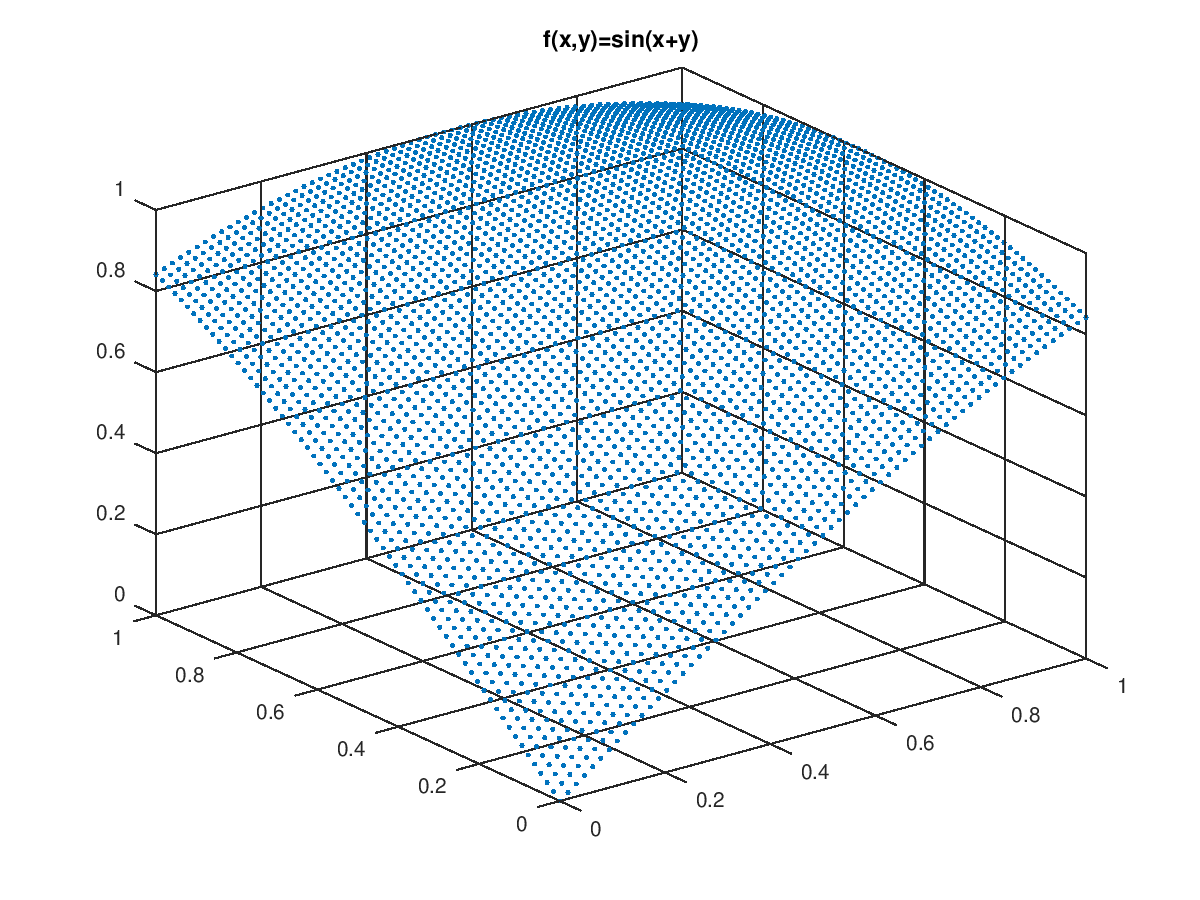
\includegraphics[width=0.8\textwidth,height=0.6\textwidth]{../output/figure/dim2_3.png}
\end{figure}

\subsection{convergence rate of error vector}
\par 通过./output/TwoDimGrid.txt中的函数error\_convergence()的输出结果看到误差向量的收敛率与残差近似,即每进行一次V-cycle,约减小一半.

\subsection{Section 9.5.1 \uppercase\expandafter{\romannumeral3}}
\begin{center}
	\begin{tabular}{|c|c|c|c|c|c|c|}
		\hline
		& $\epsilon=10^{-8}$ & $\epsilon=10^{-9}$ & $\epsilon=10^{-10}$ & $\epsilon=10^{-11}$ & $\epsilon=10^{-12}$ & $\epsilon=10^{-13}$ \\
		\hline
		V-cycle次数 & 29 & 32 & 35 & $\infty$ & $\infty$ & $\infty$ \\
		\hline
	\end{tabular}
\end{center}
当$\epsilon$下降至$10^{-11}$量级时,程序不再能达到预设的精度,这可能的原因是机器误差导致的.

\subsection{CPU time}
\par discrete\_error()函数用于计算与离散解的误差,相当于做了一次LU分解的直接求解,可以用来当作直接求解的用时。程序里将$n=128$时,对函数$e^{y+\sin(x)}$的多重网格法求解和直接求解用时进行了对比。其中设定$\epsilon=10^{-8}$,使用C++的<ctime>中的clock()函数计时.
\begin{center}
	\begin{tabular}{|c|c|c|}
		\hline
		 & V-cycle & 直接求解 \\
		 \hline
		用时 & 0.9456 & 274.898 \\
		\hline
	\end{tabular}
\end{center}
可以看到,二者运行时间的差距非常显著.



\end{large}
\end{document}